\documentclass[aspectratio=169, 10pt]{beamer}
% ==============================================================================
% Quantum Computing 12-Hour Course: Common LaTeX Beamer Preamble
% ==============================================================================
\usepackage{amsmath, amssymb, amsfonts, mathtools}
\usepackage{booktabs}
\usepackage{kotex}
\setsanshangulfont{UnDotum.ttf}[BoldFont=UnDotumBold.ttf, ItalicFont=UnDotum.ttf, BoldItalicFont=UnDotumBold.ttf]
\setmainhangulfont{UnBatang.ttf}[BoldFont=UnBatangBold.ttf, ItalicFont=UnBatang.ttf, BoldItalicFont=UnBatangBold.ttf]
\usepackage{tikz}
\usetikzlibrary{arrows.meta, positioning, shapes.geometric, calc}

% Syntax highlighting & listings
\usepackage{listings}
\usepackage{xcolor}

\definecolor{qcDarkBlue}{RGB}{20, 35, 60}
\definecolor{qcAccentBlue}{RGB}{0, 114, 206}
\definecolor{qcTeal}{RGB}{0, 168, 150}
\definecolor{qcLightGray}{RGB}{246, 248, 251}
\definecolor{qcCodeBg}{RGB}{242, 244, 247}
\definecolor{qcKeyword}{RGB}{140, 30, 120}
\definecolor{qcString}{RGB}{30, 120, 50}
\definecolor{qcComment}{RGB}{110, 110, 120}

\lstset{
    backgroundcolor=\color{qcCodeBg},
    basicstyle=\ttfamily\scriptsize,
    keywordstyle=\color{qcKeyword}\bfseries,
    stringstyle=\color{qcString},
    commentstyle=\color{qcComment},
    breaklines=true,
    showstringspaces=false,
    tabsize=4,
    frame=single,
    rulecolor=\color{qcAccentBlue!30},
    numbers=left,
    numberstyle=\tiny\color{qcComment},
    numbersep=6pt,
    xleftmargin=10pt,
    xrightmargin=5pt
}

% Beamer Theme Settings
\usefonttheme[onlymath]{serif}
\setbeamertemplate{navigation symbols}{}
\setbeamercolor{palette primary}{bg=qcDarkBlue, fg=white}
\setbeamercolor{palette secondary}{bg=qcAccentBlue, fg=white}
\setbeamercolor{palette tertiary}{bg=qcTeal, fg=white}
\setbeamercolor{structure}{fg=qcAccentBlue}
\setbeamercolor{titlelike}{parent=palette primary}
\setbeamercolor{frametitle}{bg=qcDarkBlue, fg=white}
\setbeamercolor{framesubtitle}{bg=qcDarkBlue, fg=white!85}
\setbeamerfont{frametitle}{size=\normalsize, series=\bfseries}
\setbeamerfont{framesubtitle}{size=\scriptsize, series=\normalfont}

\makeatletter
\setbeamertemplate{frametitle}{%
    \nointerlineskip%
    \begin{beamercolorbox}[wd=\paperwidth,sep=4pt,leftskip=8pt]{frametitle}%
        {\usebeamerfont{frametitle}\insertframetitle}%
        \ifx\insertframesubtitle\@empty%
        \else%
            \par\vspace{1pt}%
            {\usebeamerfont{framesubtitle}\usebeamercolor[fg]{framesubtitle}\insertframesubtitle}%
        \fi%
    \end{beamercolorbox}%
}
\makeatother

% Native Beamer Blocks (Rounded, theme-matched, 100% pause-compatible)
\setbeamertemplate{blocks}[rounded][shadow=false]

% 1. Standard block (formerly qcblock)
\setbeamercolor{block title}{fg=white, bg=qcAccentBlue}
\setbeamercolor{block body}{fg=qcDarkBlue, bg=qcLightGray}
\setbeamerfont{block title}{size=\footnotesize, series=\bfseries}

% 2. Alertblock (formerly qcalert)
\setbeamercolor{block title alerted}{fg=white, bg=red!75!black}
\setbeamercolor{block body alerted}{fg=black, bg=red!5}
\setbeamerfont{block title alerted}{size=\footnotesize, series=\bfseries}

% 3. Exampleblock (formerly qctip)
\setbeamercolor{block title example}{fg=white, bg=qcTeal}
\setbeamercolor{block body example}{fg=black, bg=green!5}
\setbeamerfont{block title example}{size=\footnotesize, series=\bfseries}

% Tight vertical block spacing
\addtobeamertemplate{block begin}{\vspace{-3pt}}{}
\addtobeamertemplate{block end}{}{\vspace{-4pt}}
\addtobeamertemplate{block alerted begin}{\vspace{-3pt}}{}
\addtobeamertemplate{block alerted end}{}{\vspace{-4pt}}
\addtobeamertemplate{block example begin}{\vspace{-3pt}}{}
\addtobeamertemplate{block example end}{}{\vspace{-4pt}}

% Backward compatibility aliases
\newenvironment{qcblock}[1]{\begin{block}{#1}}{\end{block}}
\newenvironment{qcalert}[1]{\begin{alertblock}{#1}}{\end{alertblock}}
\newenvironment{qctip}[1]{\begin{exampleblock}{#1}}{\end{exampleblock}}

% Quantum Dirac Notation Macros
\newcommand{\ket}[1]{|#1\rangle}
\newcommand{\bra}[1]{\langle#1|}
\newcommand{\braket}[2]{\langle#1|#2\rangle}
\newcommand{\ketbra}[2]{|#1\rangle\langle#2|}
\newcommand{\normsq}[1]{|#1|^2}


\title[양자컴퓨팅 부트캠프 4일차]{양자컴퓨팅 이론\&실습 4주 부트캠프}
\subtitle{4일차: QubitSquare 산업용 웹 플랫폼 종합 실습 및 결과 비교}
\author{강사: 서상협 ((주)큐렌스)}
\date{2026. 12. 04 (금)}

\begin{document}

\frame{\titlepage}

% -----------------------------------------------------------------------------
\begin{frame}{4일차 오프닝 스토리: 양자컴퓨터를 쓰고 싶은 당신이 마주친 현실}
    \begin{center}
    \begin{tikzpicture}[
        box/.style={rectangle, draw=qcDarkBlue, fill=qcLightGray, thick, rounded corners=3pt, minimum width=2.9cm, minimum height=0.9cm, font=\footnotesize\bfseries, align=center},
        arrow/.style={-{Latex[scale=0.9]}, very thick, color=qcDarkBlue}
    ]
        \node[box, fill=qcAccentBlue!15] (s1) at (0, 1.8) {1. 양자컴퓨터 활용 열망\\\scriptsize (신약/금융/최적화 연구)};
        \node[box, fill=qcTeal!15] (s2) at (4.5, 1.8) {2. 퀀텀 서킷 이해 완료\\\scriptsize (1~3일차 이론 마스터)};
        \node[box, fill=red!15, draw=red!80] (s3) at (9.0, 1.8) {3. 거대한 진입장벽!\\\scriptsize (Python, Qiskit, 가상환경)};
        \node[box, fill=orange!20, draw=orange!80, minimum width=8.5cm] (s4) at (4.5, 0.2) {\large 4. 해결책: 비(非)프로그래머를 위한 웹 GUI 플랫폼 QubitSquare!\\\scriptsize (코딩 없는 직관적 드래그 앤 드롭 \& 원클릭 시뮬레이션)};

        \draw[arrow] (s1) -- (s2);
        \draw[arrow] (s2) -- (s3);
        \draw[arrow, color=orange!80] (s3.south) -- ++(0, -0.35) -| (s4.north);
    \end{tikzpicture}
    \end{center}
    \vspace{-0.1cm}
    \begin{qcblock}{왜 우리는 GUI 플랫폼을 필요로 하는가?}
        \begin{itemize}
            \item \textbf{이론을 아는 것}과 \textbf{전문 소프트웨어 엔지니어가 되는 것}은 완전히 다른 문제입니다.
            \item 서킷 하나 돌리려고 복잡한 프로그래밍 언어의 늪(Python 문법, SDK 버전 충돌, 가상환경)에 빠져 지칠 필요가 없습니다.
            \item \textbf{QubitSquare}: 비프로그래머 연구자도 마우스 클릭만으로 양자 회로를 조립하고 즉시 실행할 수 있는 차세대 플랫폼입니다.
        \end{itemize}
    \end{qcblock}
\end{frame}

% -----------------------------------------------------------------------------
\begin{frame}{왜 QubitSquare인가? (No-Code 양자 컴퓨팅 3대 혁신)}
    \begin{qcblock}{비(非)프로그래머 및 도메인 전문가를 위한 3대 혁신}
        \begin{enumerate}
            \item \textbf{설치 없는 100\% 웹 브라우저 (Zero-Installation)}:
            파이썬, C++ 컴파일러, 패키지 설치 없이 크롬/엣지 브라우저만 열면 즉시 양자 회로를 설계합니다.
            \item \textbf{직관적인 마우스 드래그 앤 드롭 (Visual Circuit Design)}:
            수식과 교재에서 보던 게이트 기호($H, X, CX, CZ$)를 와이어 위에 그대로 끌어다 놓습니다.
            \item \textbf{올인원 파이프라인 (Design $\to$ Server Run $\to$ Compare)}:
            회로 생성부터 목적함수 설정, 서버 백엔드 실행, \textbf{결과 비교 분석(Compare)}까지 한 화면에서 완결합니다.
        \end{enumerate}
    \end{qcblock}
    \vspace{0.2cm}
    \begin{qctip}{4일차 특강의 사명}
        코딩 스트레스 없이, \textbf{순수하게 양자 알고리즘의 본질(회로 설계와 결과 분석)에만 집중}하는 실무 능력을 체득합니다.
    \end{qctip}
\end{frame}

% -----------------------------------------------------------------------------
\begin{frame}{4일차 세부 운영안 (실시간 따라하기 실습 로드맵)}
    \begin{center}
    \resizebox{0.96\textwidth}{!}{
    \begin{tikzpicture}[
        phase/.style={rectangle, draw=qcDarkBlue, fill=qcLightGray, thick, rounded corners=4pt, minimum width=4.2cm, minimum height=1.3cm, align=center, font=\small},
        arrow/.style={->, >=stealth, very thick, qcDarkBlue}
    ]
        \node[phase, fill=qcAccentBlue!15] (p1) at (0, 0) {\textbf{1부 (75분)}\\\footnotesize 기본 조작 \& Bell 회로 조립\\\scriptsize (플랫폼 접속 $\to$ 회로 조립 $\to$ 서버 100샷 실행)};
        \node[phase, fill=qcTeal!15] (brk) at (4.8, 0) {\textbf{휴식 (20분)}\\\footnotesize 두뇌 휴식 \& 계정 점검\\\scriptsize (서버 접속 확인 및 개별 에러 해결)};
        \node[phase, fill=orange!15] (p2) at (9.6, 0) {\textbf{2부 (75분)}\\\footnotesize Grover 조립 \& Compare 분석\\\scriptsize (Duplicate 복제 $\to$ Grover 실행 $\to$ 다중 대조)};

        \draw[arrow] (p1) -- (brk);
        \draw[arrow] (brk) -- (p2);
    \end{tikzpicture}
    }
    \end{center}
    \vspace{-0.1cm}
    \begin{qcblock}{실습 중심(Hands-on Driven) 운영 원칙}
        \begin{itemize}
            \item \textbf{일방적 슬라이드 강의 지양}: 강사의 화면 시연과 학생의 실시간 브라우저 조작이 1:1로 함께 진행됩니다.
            \item \textbf{100\% 서버 기반 워크플로우}: 실제 클라우드 인프라(QPlayer Compute Engine)로 회로를 전송하고 결과를 수신합니다.
            \item \textbf{수치적 비교 검증}: 100샷 vs 1,000샷의 통계 수렴(Shot Noise 감소)을 Compare 뷰에서 직접 체감합니다.
        \end{itemize}
    \end{qcblock}
\end{frame}

% -----------------------------------------------------------------------------
\begin{frame}{QubitSquare 소개 및 웹 플랫폼 접속}
    \begin{qcblock}{QubitSquare 플랫폼 개요}
        \begin{itemize}
            \item 웹 표준 기술 기반의 그래픽 양자 회로 설계 및 알고리즘 분석 플랫폼
            \item 별도 소프트웨어 설치 없이 크롬/엣지 등 최신 웹 브라우저에서 바로 구동
            \item 초심자 친화적 직관적 UI와 산업 최적화(QAOA, Max-Cut, TSP) 템플릿 내장
        \end{itemize}
    \end{qcblock}
    \vspace{0.2cm}
    \begin{qctip}{[실습 준비] 웹 브라우저 접속 및 로그인}
        \begin{enumerate}
            \item 웹 브라우저를 열고 QubitSquare 서비스 URL에 접속합니다.
            \item 배정받은 실습 계정으로 로그인합니다.
            \item 첫 화면(Dashboard / Labs)에 정상적으로 진입했는지 확인합니다.
        \end{enumerate}
    \end{qctip}
\end{frame}

% -----------------------------------------------------------------------------
\begin{frame}{QPlayer 백엔드와 서버 기반 연산 아키텍처}
    \begin{qcblock}{QPlayer 서버 API 연동 구조}
        QubitSquare는 프론트엔드 UI이며, 실제 양자 회로 연산은 \textbf{QPlayer 클라우드 서버}가 담당합니다:
    \end{qcblock}
    \begin{center}
    \begin{tikzpicture}[
        node distance=0.6cm,
        box/.style={rectangle, draw=qcDarkBlue, fill=qcLightGray, thick, rounded corners=3pt, minimum width=3.3cm, minimum height=1.0cm, align=center, font=\small},
        arrow/.style={->, >=stealth, very thick, qcDarkBlue}
    ]
        \node[box, fill=qcAccentBlue!15] (ui) {\textbf{QubitSquare UI}\\\scriptsize 회로 설계 및 파라미터};
        \node[box, fill=qcTeal!15, right=1.2cm of ui] (api) {\textbf{QPlayer API Server}\\\scriptsize 작업 수신 및 스케줄링};
        \node[box, fill=orange!20, right=1.2cm of api] (engine) {\textbf{Compute Engine}\\\scriptsize 고성능 시뮬레이터 / QPU};

        \draw[arrow] (ui) -- node[above, font=\scriptsize] {Job 제출 (Run)} (api);
        \draw[arrow] (api) -- node[above, font=\scriptsize] {작업 할당 (Queue)} (engine);
        \draw[arrow] (engine.south) -- ++(0, -0.3) -| node[above, pos=0.25, font=\scriptsize] {Result Snapshot (Counts)} (ui.south);
    \end{tikzpicture}
    \end{center}
    \vspace{-0.1cm}
    \begin{qctip}{서버 기반 실행(Server-based Execution)의 장점}
        \begin{itemize}
            \item 개인 PC의 사양(CPU/RAM)에 구애받지 않고 고성능 클라우드 자원을 활용합니다.
            \item 모든 실행 기록과 결과가 서버 DB에 영구 보존되어 언제든 재열람 및 다중 비교가 가능합니다.
        \end{itemize}
    \end{qctip}
\end{frame}

% -----------------------------------------------------------------------------
\begin{frame}{데이터와 화면의 6단계 계층 구조}
    QubitSquare의 모든 작업과 데이터는 아래 6단계 위계(Hierarchy)로 관리됩니다:
    \begin{center}
    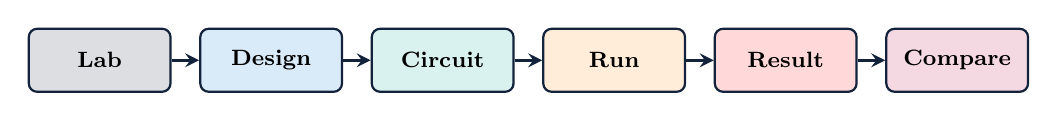
\begin{tikzpicture}[
        node distance=0.35cm,
        level/.style={rectangle, draw=qcDarkBlue, fill=qcLightGray, thick, rounded corners=3pt, minimum width=1.8cm, minimum height=0.8cm, align=center, font=\footnotesize\bfseries},
        arrow/.style={->, >=stealth, very thick, qcDarkBlue}
    ]
        \node[level, fill=qcDarkBlue!15] (l1) {Lab};
        \node[level, fill=qcAccentBlue!15, right=of l1] (l2) {Design};
        \node[level, fill=qcTeal!15, right=of l2] (l3) {Circuit};
        \node[level, fill=orange!15, right=of l3] (l4) {Run};
        \node[level, fill=red!15, right=of l4] (l5) {Result};
        \node[level, fill=purple!15, right=of l5] (l6) {Compare};

        \draw[arrow] (l1) -- (l2);
        \draw[arrow] (l2) -- (l3);
        \draw[arrow] (l3) -- (l4);
        \draw[arrow] (l4) -- (l5);
        \draw[arrow] (l5) -- (l6);
    \end{tikzpicture}
    \end{center}
    \vspace{-0.1cm}
    \begin{table}
    \centering
    \scriptsize
    \begin{tabular}{llp{9.0cm}}
    \toprule
    \textbf{단계} & \textbf{성격} & \textbf{핵심 역할 및 설명} \\
    \midrule
    \textbf{Lab} & 작업 공간 & 최상위 프로젝트 폴더 (여러 Design과 실험 내역 보관) \\
    \textbf{Design} & 설계 단위 & 회로, 목적함수 Score, 고전 최적화 루프, Display를 묶는 종합 명세 \\
    \textbf{Circuit} & 회로 에디터 & 게이트 배열 및 큐비트 와이어를 직접 편집하는 화면 \\
    \textbf{Run} & 서버 실행 & \textbf{Design 1개 $\times$ Compute Engine 1개}의 단일 작업 제출 단위 \\
    \textbf{Result} & 결과 데이터 & 실행 완료 당시의 회로 형상 스냅샷과 측정 bitstring counts \\
    \textbf{Compare} & 다중 비교 & 성공한 2~8개의 Result를 선택해 분포와 특성을 함께 대조하는 뷰 \\
    \bottomrule
    \end{tabular}
    \end{table}
\end{frame}

% -----------------------------------------------------------------------------
\begin{frame}{[실습 1-1] 워크스페이스 둘러보기 \& 5대 Puzzle Pieces}
    \begin{qcblock}{모듈식 조립판 (Design Workspace)}
        화면 좌측 조각 목록에서 중앙 조립판으로 퍼즐 조각을 드래그하여 시스템을 구성합니다:
    \end{qcblock}
    \vspace{0.2cm}
    \begin{qcblock}{5대 핵심 Puzzle Pieces}
        \begin{enumerate}
            \item \textbf{Circuit}: 기본 양자 회로를 편집하고 와이어를 배치하는 조각
            \item \textbf{Problem Source}: 그래프 가중치(Max-Cut) 또는 거리 행렬(TSP) 기반 산업 문제 소스
            \item \textbf{Score}: 측정 결과로부터 최적화 목적함수 값을 계산하는 조각
            \item \textbf{Optimizer Loop}: 파라미터 변분 양자 알고리즘(VQE, QAOA)을 위한 고전 최적화 루프
            \item \textbf{Display}: 측정 bitstring 분포 및 산업 응용 맞춤 시각화 조각
        \end{enumerate}
    \end{qcblock}
    \vspace{0.2cm}
    \begin{qctip}{[핸즈온 지침]}
        중앙 화면의 `Design` 조립판에 기본 배치된 \textbf{Circuit} 조각의 우측 상단 \textbf{‘Edit Circuit’} 버튼을 클릭해 에디터로 진입합니다.
    \end{qctip}
\end{frame}

% -----------------------------------------------------------------------------
\begin{frame}{[실습 1-2] Circuit Editor 진입 및 2-qubit Bell 회로 마우스 조립}
    \begin{qcblock}{Bell 상태 회로 구성 목표}
        Day 2에서 수식으로 유도했던 최대 얽힘 상태 $\ket{\Phi^+} = \frac{1}{\sqrt{2}}(\ket{00} + \ket{11})$를 마우스로 조립합니다:
    \end{qcblock}
    \begin{center}
    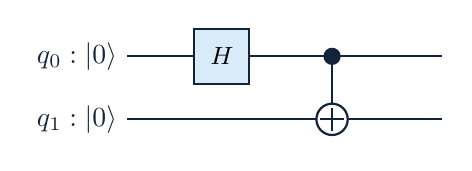
\begin{tikzpicture}[
        wire/.style={thick, color=qcDarkBlue},
        gate/.style={rectangle, draw=qcDarkBlue, fill=qcAccentBlue!15, thick, minimum size=0.7cm, font=\small\bfseries},
        dot/.style={circle, fill=qcDarkBlue, inner sep=2.2pt}
    ]
        \draw[wire] (-0.8, 0.8) node[left] {$q_0: |0\rangle$} -- (3.2, 0.8);
        \draw[wire] (-0.8, 0.0) node[left] {$q_1: |0\rangle$} -- (3.2, 0.0);

        \node[gate] at (0.4, 0.8) {$H$};
        \node[dot] at (1.8, 0.8) {};
        \draw[wire, thick] (1.8, 0.8) -- (1.8, 0.0);
        \node[circle, draw=qcDarkBlue, fill=white, thick, inner sep=4pt] at (1.8, 0.0) {};
        \draw[thick, qcDarkBlue] (1.65, 0.0) -- (1.95, 0.0);
        \draw[thick, qcDarkBlue] (1.8, -0.15) -- (1.8, 0.15);
    \end{tikzpicture}
    \end{center}
    \vspace{-0.1cm}
    \begin{qctip}{[마우스 조립 순서]}
        \begin{enumerate}
            \item 좌측 게이트 팔레트에서 \textbf{$H$ 게이트}를 마우스로 끌어 $q_0$ 와이어 첫 번째 칸에 놓습니다.
            \item \textbf{$CX$ (CNOT) 게이트}를 끌어 $q_0$ 와이어에 놓은 뒤, 타깃 연결선을 $q_1$ 와이어로 드래그합니다.
            \item 회로가 위 그림과 일치하는지 확인합니다.
        \end{enumerate}
    \end{qctip}
\end{frame}

% -----------------------------------------------------------------------------
\begin{frame}{핵심 규칙 1: 'Apply to Flow' $\neq$ 실행 (Run)}
    \begin{qcalert}{{가장 흔히 하는 실수: 'Apply to Flow'는 실행 버튼이 아닙니다!}}
        \begin{itemize}
            \item 회로 에디터 우측 상단의 \textbf{‘Apply to Flow’} 버튼은 편집한 회로를 Design 조립판에 반영하고 돌아가는 \textbf{UI 복귀/임시저장 버튼}입니다.
            \item 이 버튼을 누른다고 해서 서버로 연산 요청이 전송되거나 시뮬레이션이 실행되는 것이 아닙니다!
        \end{itemize}
    \end{qcalert}
    \vspace{0.2cm}
    \begin{qcblock}{실제 실행(Run)을 요청하는 표준 절차}
        \begin{enumerate}
            \item 회로 편집 후 \textbf{‘Apply to Flow’}를 눌러 Design Workspace로 복귀합니다.
            \item 상단 탭에서 \textbf{`Executions`} 메뉴를 클릭합니다.
            \item 연산 엔진과 shots를 지정한 뒤 우측의 \textbf{`Run`} 버튼을 눌러야 서버로 제출됩니다!
        \end{enumerate}
    \end{qcblock}
\end{frame}

% -----------------------------------------------------------------------------
\begin{frame}{핵심 규칙 2: 자동 전체 측정 (Automatic Measurement)}
    \begin{qcblock}{자동 전체 측정(Automatic Measurement) 삽입 메커니즘}
        \begin{itemize}
            \item 회로에 Measure 게이트가 \textbf{단 하나도 없으면}, QubitSquare 서버 백엔드는 실행 시 \textbf{모든 큐비트에 대한 측정을 자동으로 맨 뒤에 삽입}합니다.
            \item 명시적 Measure가 1개라도 있으면 사용자가 지정한 큐비트만 측정됩니다.
        \end{itemize}
    \end{qcblock}
    \vspace{0.3cm}
    \begin{qctip}{[실습 관찰 포인트]}
        우리가 방금 조립한 Bell 회로에는 Measure 게이트를 배치하지 않았습니다.\\
        $\implies$ 하지만 잠시 후 실행하면 자동으로 전체 측정이 적용되어 `00`과 `11` 카운트가 정상 출력됩니다!
    \end{qctip}
\end{frame}

% -----------------------------------------------------------------------------
\begin{frame}{[실습 2-1] 서버 기반 실행(Run): Compute Engine 선택 및 100 shots 제출}
    \begin{qcblock}{서버 실행 파라미터 설정}
        \begin{enumerate}
            \item 상단 네비게이션에서 \textbf{`Executions`} 탭을 클릭합니다.
            \item \textbf{Quantum Compute Engine Target}: 실습용 서버 시뮬레이터 엔진을 선택합니다.
            \item \textbf{Shots (측정 반복 횟수)}: \textbf{100}으로 설정합니다.
            \item 우측 상단의 초록색 \textbf{`Run`} 버튼을 클릭합니다!
        \end{enumerate}
    \end{qcblock}
    \vspace{0.2cm}
    \begin{qctip}{작업 큐(Queue) 상태 확인}
        \begin{itemize}
            \item 버튼을 누르면 상태가 \textbf{Pending (대기 중)} $\to$ \textbf{Running (실행 중)} $\to$ \textbf{Completed (완료)}로 전환됩니다.
            \item 서버 상에 독립된 새로운 \textbf{Run ID}가 발급되며, 완료 즉시 우측에 \textbf{`View Result`} 버튼이 활성화됩니다.
        \end{itemize}
    \end{qctip}
\end{frame}

% -----------------------------------------------------------------------------
\begin{frame}{서버 작업 처리 파이프라인: Job Submission $\to$ Result Snapshot}
    \begin{center}
    \begin{tikzpicture}[
        node distance=0.6cm,
        box/.style={rectangle, draw=qcDarkBlue, fill=qcLightGray, thick, rounded corners=3pt, minimum width=2.7cm, minimum height=0.9cm, align=center, font=\footnotesize},
        arrow/.style={->, >=stealth, very thick, qcDarkBlue}
    ]
        \node[box, fill=qcAccentBlue!15] (b1) {1. Job Submit\\\scriptsize (회로+100 shots)};
        \node[box, fill=qcTeal!15, right=of b1] (b2) {2. Server Queue\\\scriptsize (작업 스케줄링)};
        \node[box, fill=orange!20, right=of b2] (b3) {3. Simulation\\\scriptsize (상태벡터 연산)};
        \node[box, fill=green!20, right=of b3] (b4) {4. Result Snapshot\\\scriptsize (불변 데이터 생성)};

        \draw[arrow] (b1) -- (b2);
        \draw[arrow] (b2) -- (b3);
        \draw[arrow] (b3) -- (b4);
    \end{tikzpicture}
    \end{center}
    \vspace{-0.1cm}
    \begin{qcblock}{불변 스냅샷(Immutable Snapshot)의 가치}
        \begin{itemize}
            \item QubitSquare의 Result는 실행 완료 시점의 \textbf{회로 형상과 측정 카운트 데이터를 영구 스냅샷}으로 저장합니다.
            \item 이후 사용자가 Design 화면에서 회로를 마음대로 수정하더라도, 이전에 완료된 Result 스냅샷은 절대 훼손되지 않습니다!
        \end{itemize}
    \end{qcblock}
\end{frame}

% -----------------------------------------------------------------------------
\begin{frame}{[실습 2-2] Result 분석: Default Display vs Raw Distribution}
    \textbf{`View Result`}를 클릭하여 결과 화면을 열고, 우측 상단 표시 모드를 전환해 봅니다:
    \vspace{0.1cm}
    \begin{columns}[t]
        \begin{column}{0.48\textwidth}
            \begin{qcblock}{Default Display (관측 빈도 순)}
                \begin{itemize}
                    \item 실제로 \textbf{1회 이상 관측된 bitstring만} 막대그래프 축에 표시
                    \item 관측 횟수가 높은 순으로 내림차순 정렬
                    \item 최적 해답(Grover 타깃 등) 식별에 최적
                \end{itemize}
            \end{qcblock}
        \end{column}
        \begin{column}{0.48\textwidth}
            \begin{qcblock}{Raw Distribution (기저 순 4차원)}
                \begin{itemize}
                    \item 이진수 크기 순($00, 01, 10, 11$) 고정 정렬
                    \item \textbf{0회 관측된 기저 상태까지 축에 모두 표시}
                    \item 1~2일차 이론 상태벡터와 1:1 대조에 필수!
                \end{itemize}
            \end{qcblock}
        \end{column}
    \end{columns}
    \vspace{0.2cm}
    \begin{qctip}{[100 shots 실행 결과 확인]}
        Raw Distribution에서 $00$과 $11$에 약 45~55개 내외의 카운트가 찍히고, $01$과 $10$은 0개임을 확인합니다.
    \end{qctip}
\end{frame}

% -----------------------------------------------------------------------------
\begin{frame}{1부 마무리 점검 및 20분 중간 휴식 안내}
    \begin{qcblock}{1부 실습 달성도 체크}
        \begin{itemize}
            \item $\checkmark$ QubitSquare 웹 플랫폼 접속 및 서버 계정 로그인 완료
            \item $\checkmark$ 2-qubit Bell 회로 마우스 드래그 앤 드롭 조립
            \item $\checkmark$ 'Apply to Flow' $\neq$ Run 규칙 및 자동 전체 측정 메커니즘 체득
            \item $\checkmark$ QPlayer 서버로 100 shots Run 제출 및 Result 스냅샷 생성 확인
        \end{itemize}
    \end{qcblock}
    \vspace{0.3cm}
    \begin{qctip}{20분간 중간 휴식 및 개별 점검}
        \begin{itemize}
            \item 두뇌 휴식을 취하며, 서버 접속 오류나 실행 지연이 있는 분은 강사에게 질문해 주세요.
            \item 2부에서는 \textbf{Grover 회로 조립, 1,000 shots 실행, 그리고 대망의 Compare 다중 비교}가 이어집니다!
        \end{itemize}
    \end{qctip}
\end{frame}

% -----------------------------------------------------------------------------
\begin{frame}{2부 오프닝: 심화 회로 조립 및 Compare 다중 분석 로드맵}
    \begin{qcblock}{2부 실습 미션 (75분)}
        \begin{enumerate}
            \item \textbf{Duplicate 기능 활용}: 기존 Bell Design을 복제하여 안전하게 새 실험 분기 생성
            \item \textbf{2-qubit Grover 회로 조립}: Phase Oracle과 Diffusion 연산자를 마우스로 조립
            \item \textbf{1,000 shots 서버 제출}: 샷 수를 10배 늘려 정밀 실행
            \item \textbf{Compare 탭 다중 분석 (핵심)}: 100 shots vs 1,000 shots를 나란히 비교하여 \textbf{Shot Noise 통계 수렴}을 실증적으로 확인
            \item \textbf{산업 템플릿 탐색}: Max-Cut 및 TSP 템플릿 로드 및 회로 변환 구경
        \end{enumerate}
    \end{qcblock}
\end{frame}

% -----------------------------------------------------------------------------
\begin{frame}{핵심 규칙 3: 실험 분기를 위한 Design Duplicate 복제}
    \begin{qcalert}{{주의: 기존 Design의 회로를 그냥 덮어쓰지 마세요!}}
        \begin{itemize}
            \item 동일한 Design에서 회로를 지우고 새로 그리면, 이전 실험과의 맥락적 연결이 복잡해질 수 있습니다.
            \item 새로운 알고리즘(Grover)이나 다른 파라미터를 테스트할 때는 상단의 \textbf{`Duplicate`} 버튼을 사용하는 것이 표준입니다.
        \end{itemize}
    \end{qcalert}
    \vspace{0.2cm}
    \begin{qcblock}{Duplicate 복제의 이점}
        \begin{itemize}
            \item 현재 Design의 모든 설정(회로, 목적함수, Display)이 완전히 독립된 새 Design으로 복제됩니다.
            \item 원본 Bell Design은 그대로 보존되므로, 나중에 \textbf{Compare 탭에서 Bell 결과와 Grover 결과를 동시에 불러와 비교}할 수 있습니다!
        \end{itemize}
    \end{qcblock}
\end{frame}

% -----------------------------------------------------------------------------
\begin{frame}{[실습 3-1] Duplicate 복제 및 2-qubit Grover 회로 마우스 조립}
    \begin{qcblock}{[핸즈온 단계]}
        \begin{enumerate}
            \item 상단 `Design` 화면에서 \textbf{`Duplicate`}를 클릭하여 새 Design을 생성하고 이름을 `Grover-2Q`로 변경합니다.
            \item Circuit 조각의 \textbf{‘Edit Circuit’}을 누르고 기존 게이트를 삭제합니다.
            \item 3일차에 배운 2-qubit Grover 회로(타깃 $|11\rangle$)를 마우스로 조립합니다:
        \end{enumerate}
    \end{qcblock}
    \begin{center}
    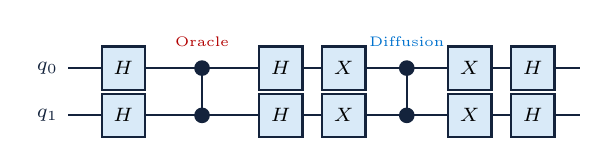
\begin{tikzpicture}[
        wire/.style={thick, color=qcDarkBlue},
        gate/.style={rectangle, draw=qcDarkBlue, fill=qcAccentBlue!15, thick, minimum size=0.55cm, font=\scriptsize\bfseries},
        dot/.style={circle, fill=qcDarkBlue, inner sep=2.0pt}
    ]
        \draw[wire] (-0.5, 0.6) node[left] {\scriptsize $q_0$} -- (6.0, 0.6);
        \draw[wire] (-0.5, 0.0) node[left] {\scriptsize $q_1$} -- (6.0, 0.0);

        \node[gate] at (0.2, 0.6) {$H$};
        \node[gate] at (0.2, 0.0) {$H$};

        % Oracle CZ
        \node[dot] at (1.2, 0.6) {};
        \node[dot] at (1.2, 0.0) {};
        \draw[wire, thick] (1.2, 0.6) -- (1.2, 0.0);
        \node[above, font=\tiny, color=red!70!black] at (1.2, 0.75) {Oracle};

        % Diffusion
        \node[gate] at (2.2, 0.6) {$H$};
        \node[gate] at (2.2, 0.0) {$H$};
        \node[gate] at (3.0, 0.6) {$X$};
        \node[gate] at (3.0, 0.0) {$X$};
        \node[dot] at (3.8, 0.6) {};
        \node[dot] at (3.8, 0.0) {};
        \draw[wire, thick] (3.8, 0.6) -- (3.8, 0.0);
        \node[gate] at (4.6, 0.6) {$X$};
        \node[gate] at (4.6, 0.0) {$X$};
        \node[gate] at (5.4, 0.6) {$H$};
        \node[gate] at (5.4, 0.0) {$H$};
        \node[above, font=\tiny, color=qcAccentBlue] at (3.8, 0.75) {Diffusion};
    \end{tikzpicture}
    \end{center}
    \vspace{-0.2cm}
    \begin{center}
        \footnotesize \textbf{‘Apply to Flow’}를 클릭하여 Design 화면으로 복귀합니다.
    \end{center}
\end{frame}

% -----------------------------------------------------------------------------
\begin{frame}{[실습 3-2] 1,000 shots 상향 설정 및 서버 2차 Run 제출}
    \begin{qcblock}{서버 정밀 실행 요청}
        \begin{enumerate}
            \item 상단 \textbf{`Executions`} 탭으로 이동합니다.
            \item 방금 생성한 \textbf{`Grover-2Q`} Design이 선택되어 있는지 확인합니다.
            \item 이번에는 통계적 정밀도를 높이기 위해 Shots를 \textbf{1,000}으로 상향 설정합니다!
            \item 초록색 \textbf{`Run`} 버튼을 클릭하여 서버로 2차 연산을 제출합니다.
        \end{enumerate}
    \end{qcblock}
    \vspace{0.2cm}
    \begin{qctip}{Result 확인}
        \begin{itemize}
            \item 상태가 Completed로 바뀌면 \textbf{`View Result`}를 클릭합니다.
            \item 단 1회의 Grover 반복만으로 타깃 기저인 \textbf{`11`이 1,000회 중 1,000회(100\%) 검출}되는 기적적인 양자 간섭 결과를 직접 확인합니다!
        \end{itemize}
    \end{qctip}
\end{frame}

% -----------------------------------------------------------------------------
\begin{frame}{QubitSquare Result 데이터의 본질: 샷 관측 카운트와 엔디언}
    \begin{qcblock}{복소 상태벡터 vs 샷 관측 카운트(Counts)}
        \begin{itemize}
            \item Day 1~2의 상태벡터 $\ket{\psi}$는 측정 전 닫힌계의 복소 진폭이었습니다.
            \item QubitSquare Result는 물리적 측정 후의 \textbf{고전 관측 빈도(Counts)}입니다. 플랫폼은 측정 확률에 비례하여 난수 샘플링된 실제 실험 데이터를 제공합니다.
        \end{itemize}
    \end{qcblock}
    \vspace{0.2cm}
    \begin{qctip}{비트 순서(Endianness) 주의점}
        \begin{itemize}
            \item \textbf{Qiskit Little-Endian}: $|q_1 q_0\rangle$ (맨 오른쪽이 $q_0$)
            \item \textbf{QubitSquare}: 화면 상단부터 $q_0, q_1$ 순으로 배치되므로, 출력 bitstring의 각 자리수가 어떤 큐비트의 측정값인지 대조할 때 인덱스 순서를 명확히 숙지합니다.
        \end{itemize}
    \end{qctip}
\end{frame}

% -----------------------------------------------------------------------------
\begin{frame}{[실습 4-1] Compare 조각: 성공한 다중 Result 나란히 대조}
    QubitSquare의 가장 강력한 분석 기능인 \textbf{`Compare`}를 실행합니다:
    \vspace{0.2cm}
    \begin{qcblock}{Compare 뷰 생성 방법}
        \begin{enumerate}
            \item 상단 메뉴의 \textbf{`Compare`} 탭으로 이동하거나, Puzzle Pieces에서 Compare 조각을 엽니다.
            \item 결과 목록에서 앞서 실행 완료된 결과들을 체크합니다:
            \begin{itemize}
                \item Result 1: Bell 상태 (100 shots)
                \item Result 2: Bell 상태 (추가 1,000 shots 실행본이 있는 경우)
                \item Result 3: Grover-2Q 상태 (1,000 shots)
            \end{itemize}
            \item \textbf{‘Generate Comparison’}을 클릭하면 한 화면에 다중 히스토그램이 나란히 렌더링됩니다!
        \end{enumerate}
    \end{qcblock}
\end{frame}

% -----------------------------------------------------------------------------
\begin{frame}{[실습 4-2 분석] Shot Noise 수렴 비교: 100 shots vs 1,000 shots}
    \begin{qcblock}{교육적 비교 포인트 1: 유한 샘플링 오차(Shot Noise)의 체감}
        \begin{itemize}
            \item \textbf{Bell (100 shots)}:
            이론적 확률은 50:50이지만, 실제 측정값은 47:53, 44:56 등 통계적 요동(Fluctuation)이 발생합니다.
            \item \textbf{Bell (1,000 shots)}:
            표본 수가 10배 늘어남에 따라 49.8:50.2 등 이론적 50\%에 훨씬 가깝게 수렴합니다.
        \end{itemize}
    \end{qcblock}
    \vspace{0.3cm}
    \begin{qctip}{양자 실험 설계의 실무적 교훈}
        양자 컴퓨터는 확률적 기기이므로, \textbf{도메인 문제에서 요구하는 신뢰도에 맞추어 적절한 Shots 수를 설계하는 역량}이 왜 필수적인지를 Compare 화면을 통해 시각적으로 입증합니다.
    \end{qctip}
\end{frame}

% -----------------------------------------------------------------------------
\begin{frame}{[실습 4-3 분석] 알고리즘 특성 비교: Bell 얽힘 vs Grover 증폭}
    \begin{qcblock}{교육적 비교 포인트 2: 양자 상태의 본질적 차이 한눈에 대조}
        \begin{itemize}
            \item \textbf{Bell 상태 히스토그램}:
            두 개의 명확한 기저($00$과 $11$)가 정확히 절반씩 양분되는 \textbf{완전 얽힘(Entanglement)}의 특성을 보입니다.
            \item \textbf{Grover 상태 히스토그램}:
            오직 단 하나의 정답 기저($11$)에 100\% 확률이 압도적으로 집중되는 \textbf{상쇄 간섭 기반 양자 증폭(Quantum Amplification)}의 정수를 보여줍니다.
        \end{itemize}
    \end{qcblock}
    \vspace{0.3cm}
    \begin{qctip}{Compare의 진정한 가치}
        숫자 표나 단일 그래프로는 파악하기 힘든 알고리즘 간의 거시적 통계 형태를 한눈에 직관적으로 비교할 수 있습니다.
    \end{qctip}
\end{frame}

% -----------------------------------------------------------------------------
\begin{frame}{[실습 5-1] 산업 문제 템플릿 탐색: Max-Cut (네트워크 분할)}
    QubitSquare는 순수 게이트 조작을 넘어 실제 산업 최적화 문제를 다루는 전용 템플릿을 내장하고 있습니다:
    \vspace{0.2cm}
    \begin{qcblock}{Conflict-Aware Network Segmentation (Max-Cut)}
        \begin{itemize}
            \item 네트워크 서버 노드 간의 통신 충돌 가중치를 그래프 GUI에서 마우스로 직접 편집합니다.
            \item 내부적으로 QAOA(양자 근사 최적화) 서킷 및 Score 조각이 자동 연결됩니다.
            \item 실행 후 Result에서 네트워크가 두 그룹(빨강/파랑)으로 최적 분할된 시각화 결과를 열람합니다.
        \end{itemize}
    \end{qcblock}
    \vspace{0.2cm}
    \begin{qctip}{[핸즈온 지침]}
        Templates 메뉴에서 `Network Segmentation`을 열고 그래프 노드를 클릭해 가중치를 변경해 봅니다.
    \end{qctip}
\end{frame}

% -----------------------------------------------------------------------------
\begin{frame}{[실습 5-2] 산업 문제 템플릿 탐색: TSP \& 'Convert to gates'}
    \begin{qcblock}{Shortest Cycle Route Optimization (TSP - 외판원 순회)}
        \begin{itemize}
            \item 여러 도시 간의 거리 행렬(Distance Matrix) 표를 화면에서 편집합니다.
            \item 최적 순회 경로가 TSP Route Display 지도 위에 시각적으로 렌더링됩니다.
        \end{itemize}
    \end{qcblock}
    \vspace{0.2cm}
    \begin{qcalert}{{'Convert to gates' 기능 사용 시 주의사항}}
        \begin{itemize}
            \item 템플릿 우측의 \textbf{'Convert to gates'}를 누르면 블랙박스 템플릿이 수십 개의 개별 게이트 회로로 분해되어 와이어에 전개됩니다.
            \item \textbf{비가역적(Irreversible) 작업}: 한 번 게이트로 분해하고 나면 템플릿의 자동 수식 동기화가 해제되므로 주의해야 합니다!
        \end{itemize}
    \end{qcalert}
\end{frame}

% -----------------------------------------------------------------------------
\begin{frame}{12시간 특강 종합 수료식: 선형대수에서 산업용 플랫폼까지}
    \begin{center}
        \Large \color{qcDarkBlue} \textbf{선형대수학 $\implies$ NumPy $\implies$ Qiskit $\implies$ QubitSquare}
    \end{center}
    \vspace{0.1cm}
    \begin{table}
    \centering
    \scriptsize
    \begin{tabular}{llp{9.2cm}}
    \toprule
    \textbf{단계} & \textbf{핵심 개념} & \textbf{우리가 정복한 역량} \\
    \midrule
    \textbf{Day 1} & 단일 큐비트 & 상태는 복소 열벡터 $\ket{\psi}$이며, 단일 게이트는 유니터리 행렬곱임을 손계산과 NumPy로 정복 \\
    \textbf{Day 2} & 다중 큐비트 & 텐서곱($\otimes$)과 CNOT을 통해 얽힘(Bell 상태)을 합성하고 부분 측정을 시뮬레이션 \\
    \textbf{Day 3} & 알고리즘 & 위상 킥백과 상쇄 간섭을 설계하여 Grover 탐색으로 타깃을 100\% 검출 \\
    \textbf{Day 4} & 산업 플랫폼 & No-Code 웹 GUI QubitSquare에서 서버 실행과 Compare로 실무 분석 역량 완성 \\
    \bottomrule
    \end{tabular}
    \end{table}
    \vspace{0.2cm}
    \begin{center}
        \textbf{12시간 동안 수고 많으셨습니다! 여러분은 이제 수학과 플랫폼으로 양자컴퓨팅을 다룰 수 있습니다.}
    \end{center}
\end{frame}

\end{document}
